%%%%%%%%%%%%%%%%%%%%%%%%%%%%%%%%%%%%%%%%%
% Stylish Article
% LaTeX Template
% Version 2.1 (1/10/15)
%
% This template has been downloaded from:
% http://www.LaTeXTemplates.com
%
% Original author:
% Mathias Legrand (legrand.mathias@gmail.com) 
% With extensive modifications by:
% Israel Aguilera  (israel.aguilera.navarrete@gmail.com) Nov. 2022
%
% License:
% CC BY-NC-SA 3.0 (http://creativecommons.org/licenses/by-nc-sa/3.0/)
%
%%%%%%%%%%%%%%%%%%%%%%%%%%%%%%%%%%%%%%%%%

%----------------------------------------------------------------------------------------
%	PACKAGES AND OTHER DOCUMENT CONFIGURATIONS
%----------------------------------------------------------------------------------------

\documentclass[fleqn,10pt]{AmateCodex} % Document font size and equations flushed left

\usepackage[activeacute,spanish]{babel}

\fancyhead[R]{{\textsf{DOI-http-2036}}\\
      {{\textsf{Agosto Diciembre, 2022. M\'{E}XICO}}}}
\fancyfoot[L]{{{Tlamatque \textbf{ISSN-xxx-xxx}}}}
\fancyfoot[C]{{{\textsf{P \'{a} g i n a \textbar  \textbf{\thepage} }}}}
\fancyfoot[R]{
\includegraphics[width=2cm]{imagenes/LOGO-Tlamatque2.pdf}}

%----------------------------------------------------------------------------------------
%	HYPERLINKS
%----------------------------------------------------------------------------------------

\usepackage{hyperref} % Required for hyperlinks
\hypersetup{hidelinks,colorlinks,breaklinks=true,urlcolor=blue,citecolor=blue,linkcolor=blue,bookmarksopen=false,pdftitle={Title},pdfauthor={Author}}

%----------------------------------------------------------------------------------------
%	ARTICLE INFORMATION
%----------------------------------------------------------------------------------------

\JournalInfo{Tlamatque, Vol. XXI, No. 1, 1-5, 2022} % Journal information
\Archive{DOI- htt -2036} % Additional notes (e.g. copyright, DOI, review/research article)

\PaperTitle{Lobo feroz induce a Caperucita por la vía larga, mientras éste se transporta a través de la vía corta, produciendo fagocitosis de abuelita y caperucita, las cuales son rescatadas de este destino por cazador} % Article title

\Authors{Sebastián Ewoldt\textsuperscript{1,}\textsuperscript{2}*, Ignacio Gran\textsuperscript{2,}\textsuperscript{3}} % Authors
\affiliation{\textsuperscript{1}\textit{Departamento de estudios basados en Ortomoléculas con Escleroproteínas Hidrolizadas, Felixe University of Chemistry and
Kinetics, FUCK, Santiago de Chile.}} % Author affiliation
\affiliation{\textsuperscript{2}\textit{Departamento de Diagnósticos y Tratamientos Médico-Nucleares, Astrofísicos y cuánticos, Soc. Benéfica Dr. Jorge Castro de La Barra, Chile}} % Author affiliation
\affiliation{\textsuperscript{3}\textit{Departamento de Estudios Moleculares basados en Novelas Infantiles, Pontificia Universidad Católica de Chile}} % Author affiliation
\affiliation{*\textbf{Autor de correspondencia}: siewoldt@uc.cl} % Corresponding author

\date{Recibido: \today / Aceptado: 18 marzo 2023}

\Keywords{cuentos infantiles --- caperucita --- lobo feroz} % Keywords - if you don't want any simply remove all the text between the curly brackets  , , , abuelita, frutas, silvestre, induce, ocio.
\newcommand{\keywordname}{Keywords} % Defines the keywords heading name

%----------------------------------------------------------------------------------------
%	ABSTRACT
%----------------------------------------------------------------------------------------
\Abstract{Caperucita lleva frutas diariamente en su canasta a su abuelita. En este trabajo comprobamos que caperucita elige constitutivamente la vía corta, pero en presencia de un lobo feroz se induce una elección por la vía larga. Además, aprovechando el curso temporal retrasado de la incorporación de caperucita a la casa de la abuelita, lobo feroz fagocita a esta última y expresa marcadores de superficie característicos de abuelita. Lobo feroz expresando marcadores de abuelita logra imitar con similar eficacia a los efectos de la abuelita original en caperucitas sanas. Esta interacción permite la fagocitosis de caperucita por lobo feroz. Adicionalmente, la incorporación de un cazador al medio termina con la lisis de lobo feroz y la liberación de caperucita y abuelita intactas.}
%----------------------------------------------------------------------------------------

\begin{document}

\flushbottom % Makes all text pages the same height
\maketitle % Print the title and abstract box
\tableofcontents % Print the contents section
\thispagestyle{empty} % Removes page numbering from the first page


%----------------------------------------------------------------------------------------
%	ARTICLE CONTENTS
%----------------------------------------------------------------------------------------

\section{Introduction} % The \section*{} command stops section numbering

Los fenómenos de transporte de frutas silvestres (FS) entre casa de caperucita y abuelita ocurren constitutivamente durante todo el año \cite{Guardabosques01}, pero son upregulados durante la estación fría, probablemente inducidos por episodios de enfermedad de la abuelita \cite{Lenador01}. 
Este tema ha sido parcialmente estudiado, y en la actualidad, dentro de nuestros datos, se conocen 2 rutas por las que el transporte puede ocurrir. La primera, denominada vía corta, es la más estudiada de ambas, y es la ruta de elección para el transporte de FS durante todos los ciclos \cite{Pedofilo01}. 
La segunda ruta, denominada vía larga, tiene una desconocida importancia en estos fenómenos y no se registran
trabajos concluyentes sobre el tema. Sin embargo, reportes recientes sugieren una importancia de esta
ruta en las interacciones lobo feroz-caperucita, aunque no existe claridad en el asunto. Además,
trabajos de Guardabosques y su equipo \cite{Guardabosques02} indican que lobo feroz compite con caperucita por la ruta
corta. Estos hallazgos, sumados a una falla de caperucita por seguir la ruta corta cuando lobo feroz
está ocupándola, nos han hecho proponer la hipótesis de que lobo feroz induce la elección de caperucita
por la ruta larga, por tanto siendo un elemento clave en la regulación de tráfico en el bosque, el cual
permanece como un fenómeno bastante desconocido.

%------------------------------------------------
\section{Materiales y métodos}
\subsection{Animales}
Lobo feroz, macho $(80 Kg)$ fue criado bajo condiciones estándar de lobos, descritas anteriormente \cite{Herret}
. Para el experimento de inducción, lobo feroz fue incorporado en el medio de manera espontánea, en el momento previo al \textit{comitted step} de cualquiera de ambas vías.

Para el detectar el cambio de fenotipo se utilizó lobo feroz wild-type en un grupo, en contraste a lobo
feroz 5 minutos post fagocitosis de abuelita. En ambos grupos se agregó caperucita para evidenciar
los efectos abuelitamiméticos. Se incubaron durante cinco minutos y se realizaron las observaciones.
No se respetó ningún protocolo de bienestar animal.
Lobo feroz fue cruelmente destruido en todos los experimentos por el agente cazador, sin respeto
alguno a tratados internacionales, grupos ecologistas o minas sensibles y pseudosensibles que pretendan
ganar adeptos defendiendo causas nobles y animalísticas que en realidad no le importan.


\subsection{Frutas Silvestres}
Las FS fueron generosamente donadas por "Mamá de Caperucita", puestas en una canasta y conjugadas
con caperucita previamente a cualquier experimento.

\subsection{Cazador:}
Cazador fue recolectado directamente del bosque.
Corresponde a un ejemplar solitario y sin ningún talento, dedicado a vagar en espera de algún acontecimiento importante, y desdichado desde que su última novia lo dejara por otro más viril \cite{Ependorf}.

\subsection{Reactivos}
Caperucita y abuelita fueron compradas en un infomercial fome. Garantía de satisfacción de 1 mes o le devolvemos su dinero.

\subsection{Bosques:}
Debido a la carencia de bosques naturales, se construyó un sistema in vitro con flores de vidrio y pasto artificial. Se usaron niños de entre 4 y 6 años de edad disfrazados de árboles $(n = 17)$ de los cuales 3 se retiraron del experimento por voluntad propia y 2 murieron asfixiados por el disfraz (datos no mostrados) y uno fue accidentalmente talado con
una motosierra.

\subsection{Determinación de la inducción lobo-caperucita}
Se realizaron tres experimentos en cada grupo. 
El grupo control consistió en la incorporación del conjugado caperucita-complejo canasta/FS (CCCCFS) al bosque ya descrito. Se determinó la ruta escogida en base a la lectura de las frases del narrador. En el grupo experimental se agregó CCCCFS + Lobo Feroz (LF) al mismo bosque. 
La determinación de resultados se realizó de la misma manera que en el grupo control. Se consideró resultado exitoso una observación del narrador indicando que caperucita optó por el camino largo.

\subsection{Determinación de fagocitosis de abuelita}
Para determinar con certeza la fagocitosis de la abuelita, se midió el consumo de oxígeno antes y después de la incorporación de LF a la casa de la abuelita. Se esperaron 5 minutos y se realizó otra medición. Para verificar este hecho, posteriormente a la lisis del lobo y recuperación de la abuelita intacta, se procedió a incubar abuelita + CCCCFS para determinar su interacción y compararla con las descripciones típicas de \cite{Guardabosques01}.

\subsection{Determinación del cambio de fenotipo de lobo
feroz}
En un grupo control se incubó lobo feroz wild type
(LF-WT) + CCCCFS. Mientras que en el grupo
experimental se incubó CCCCFS + Lobo feroz
postprandial (LF-PP). Se evidenciaron los resultados
a través de las preguntas de CCCFS a LF-WT y LF-
PP, según corresponda, información obtenida a
través del narrador.

\subsection{Determinación de Lisis de LF-PP}
30 minutos después de la incorporación de cazador,
se incubó la casa de la abuelita con anticuerpos anti
tripas de lobo (anticuerpo primario, Cortesía de
antianticuerpos antisociales Antígona ltda, Enrique
Segoviano 1342.). Posteriormente, se realizó un
lavado de la casa (mayordomos profesionales
Nelson) y se volvió a incubar con un anticuerpo
secundario antianticuerpoantitripas
de
lobo,
conjugado con aceite de tractor (Ricomer, servicios
de alimentación y mecánica de maquinaria agrícola).
Después de un segundo lavado se guardó la solución
contenida en la casa. Este procedimiento se repitió
exactamente en un grupo control (LF-PP sin
cazador). Las soluciones obtenidas fueron
administradas por vía oral a Huemules Chilenos
(hippocamelus bisulcus) y se cuantificaron los
decesos en ambos grupos. La concentración de
aceite de tractor en cada solución estaría relacionada
de manera directamente proporcional, en último
término, a la presencia de tripas expuestas de lobo,
por tanto, los efectos de la ingesta crónica de aceite
de tractor, descritos como obesidad, dislipidemia,
reprobación de ramos anuales, rotura de relojes y
muerte \cite{Guaton} pueden observarse en los huemules, y por
tanto, existe una correlación importante entre el
número de decesos por grupo y la lisis de lobos en el
mismo experimento.

\subsection{Final feliz}
El final feliz es asumido debido a que los cuentos
infantiles no saben hacer otra cosa \cite{Conocimientoc}.
Figura \ref{fig:Caperucita-Fig01}.

\begin{figure}[h]\centering
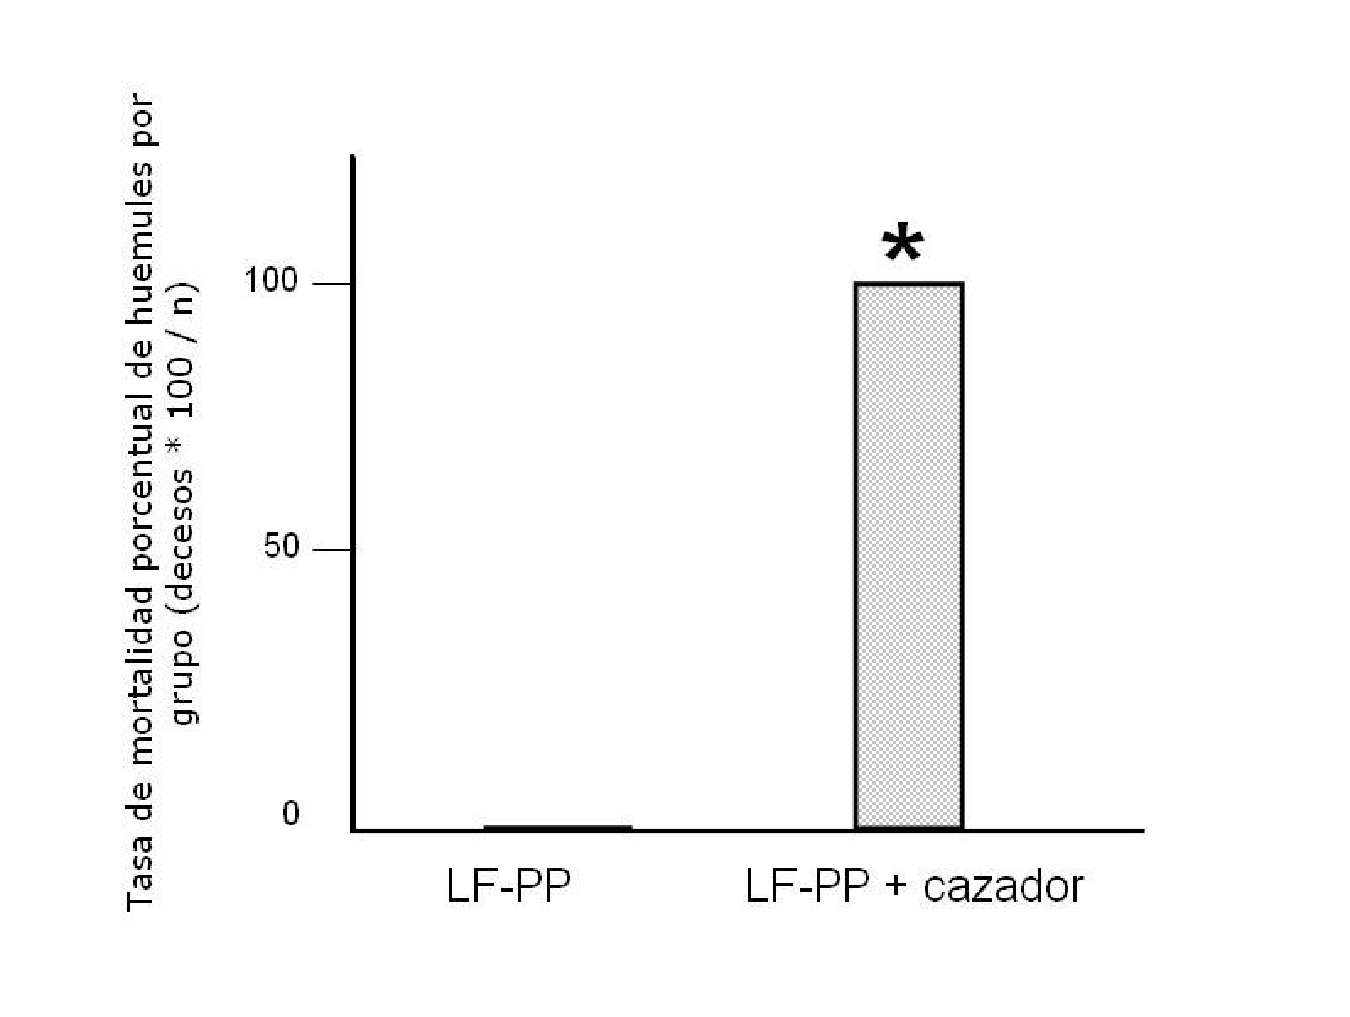
\includegraphics[width=\linewidth]{imagenes/Caperucita-Fig01.png}
\caption{Tasa de mortalidad porcentual de huemules por grupos. No se registró mortalidad en el grupo $LF-PP$ ($n = 23$).Por el contrario, en el grupo $LF-PP + cazador$ $(n = 24)$, se registraron 24 decesos, correspondientes al $100\%$ de lapoblación de ese grupo.}
\label{fig:Caperucita-Fig01}
\end{figure}

\subsection{Análisis estadístico}
Se utilizó la calculadora Casio CFX-9850 GB Plus
para los análisis estadísticos. Se consideran
diferencias significativas a partir de un valor $p<0.05$.


%------------------------------------------------
\section{Discusión}
A pesar de las valiosas contribuciones de los citados
autores en el tema del transporte de FS en el bosque,
las interacciones y mecanismos que lo gobiernan aún
no han sido dilucidados. Figura \ref{fig:Caperucita-Fig02}.

\begin{figure}[h]\centering
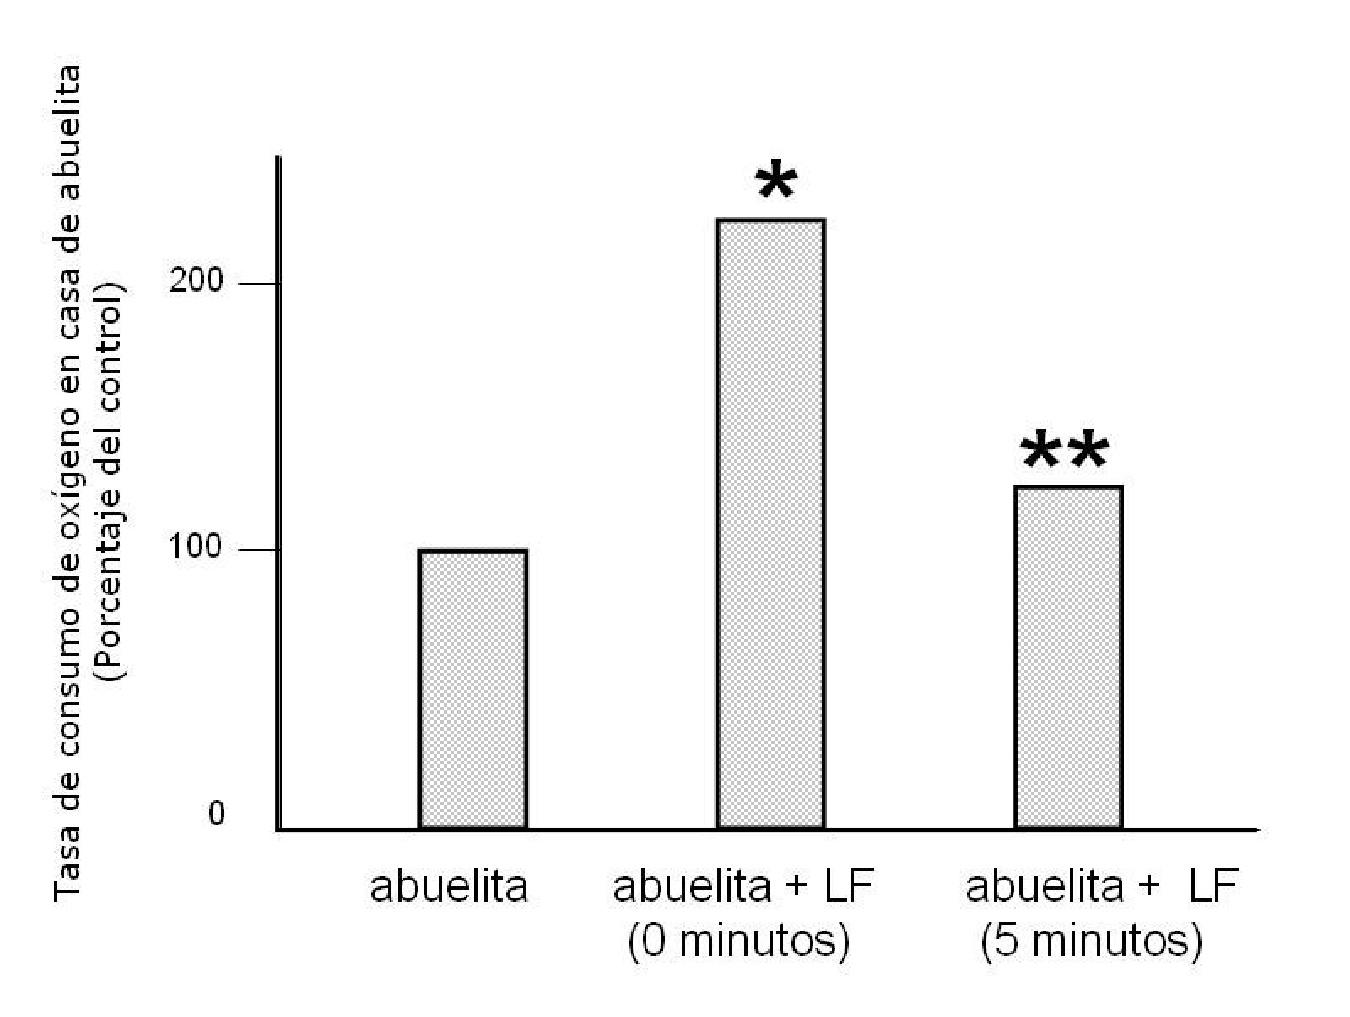
\includegraphics[width=\linewidth]{imagenes/Caperucita-Fig02.png}
\caption{Tasa de consumo de oxígeno en casa de la abuelita. Resultados expresados como porcentaje del control: En el grupo abuelita + LF, al instante 0 a partir de la adición de LF, se registró un consumo de oxígeno de más de dos veces el control. En el mismo grupo, en mediciones cinco minutos después se registró un consumo de oxígeno cercano al $100\%$ del control. *: Diferencia significativa respecto al control, **: Diferencia significativa respecto al mismo grupo en el experimento anterior, pero no significativa respecto al control.}
\label{fig:Caperucita-Fig02}
\end{figure}


\begin{figure*}[ht]\centering % Using \begin{figure*} makes the figure take up the entire width of the page
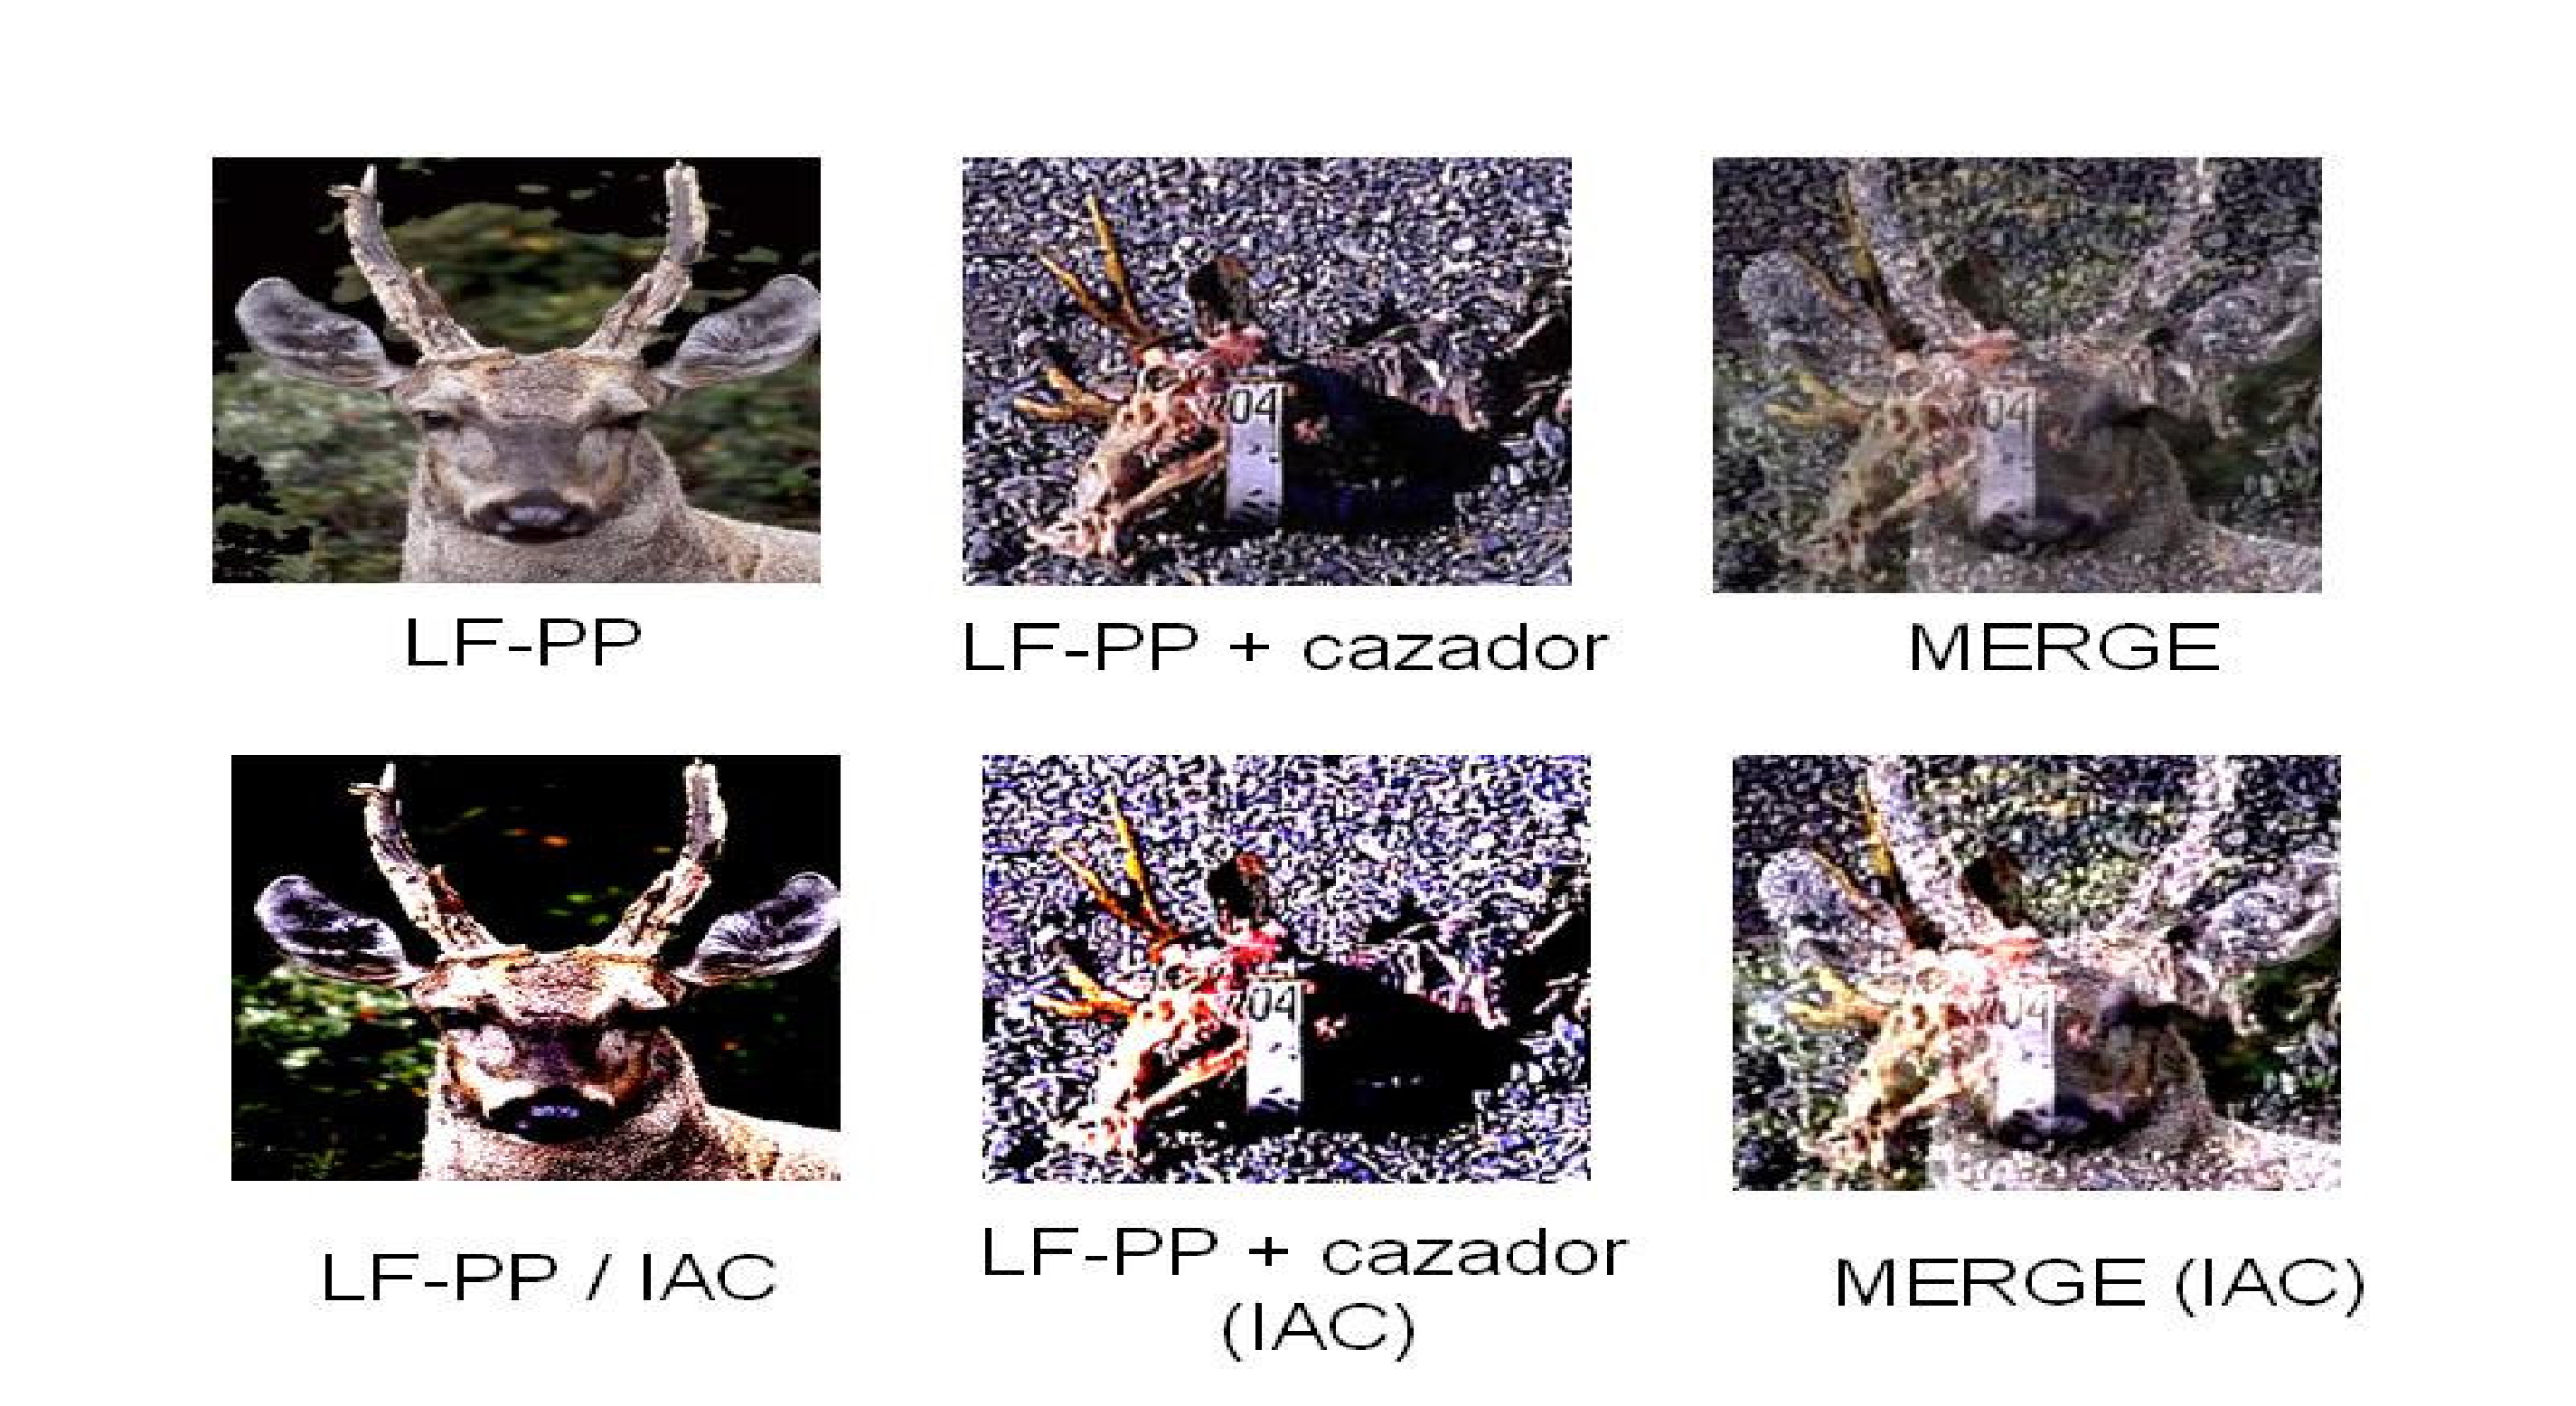
\includegraphics[width=\linewidth]{imagenes/Caperucita-Fig03.png}
\caption{Colecciones de píxeles representativas de los grupos del experimento de lisis de lobo. LF-PP: Se muestra una imagen de un huemul del grupo LF-PP durante el experimento. LF-PP + cazador: Se muestra una imagen de un huemul del grupo LF-PP + cazador, fallecido durante el experimento. Merge: Se muestran ambas imágenes superpuestas. En la fila inferior se muestra la misma tira de imágenes, esta vez procesadas con técnica IAC: Imagen de alto contraste.}
\label{fig:Caperucita-Fig03}
\end{figure*}

Nuestro trabajo arroja las primeras luces sobre los
factores que determinan la ruta que sigue caperucita
en su recorrido en el bosque, y probablemente
contribuirá a la mejor comprensión de esta vía poco
estudiada. Los resultados del experimento 1
muestran que la presencia de lobo feroz en el
bosque, logró enviar a caperucita por el camino
largo, opción que bajo condiciones normales nunca
es elegida espontáneamente. Queda pendiente la
razón de esta interacción, aunque proponemos que
esta inducción es un mecanismo adaptativo del lobo,
que pretende darle ventaja sobre caperucita, para
permitirle llegar a la casa de la abuelita antes que
caperucita. Pensamos esto debido a que, a pesar de
su nombre, el lobo feroz no goza de ferocidad, y
pareciera ser bastante cobarde. Es por esto que
podría preferir permanecer oculto y atacar por
sorpresa, que confrontarse directamente con
caperucita, situación en la que podría salir dañado.
Un inconveniente en nuestra teoría es que los lobos
son significativamente más rápidos que caperucita,
por tanto, la decisión en los caminos es un asunto
totalmente innecesario.

El primer peak en el consumo de oxígeno del
experimento dos, puede explicarse por la aparición
del lobo en la casa de la abuelita, duplicando el
consumo de oxígeno, debido a la simple presencia de
un individuo extra. La posterior caída en el consumo
de oxígeno puede explicarse por la fagocitosis de la
abuelita, la cual, a nuestro parecer, deja de respirar
mientras se encuentra en el interior del lobo, pero no
pierde su vida. La reacción positivamente
identificada como abuelita-caperucita en el final del
experimento, demuestra que la abuelita sigue viva y
su fenotipo no ha cambiado después de haber sido
fagocitada y rescatada.

El cambio de fenotipo es evidente en el experimento
3. Queda claro que caperucita es lo suficientemente
inteligente para distinguir un lobo de su abuelita, en
condiciones normales, pero que es engañada
burdamente por un lobo postprandial. De esto se
desprende que: o la imitación de abuelita del lobo es
muy precisa, o bien, caperucita es una pobre tipa
incapaz de diferenciar un lobo disfrazado de la
madre de su madre.

La preguntas que caperucita realiza al lobo sugieren
que los efectos abuelitamiméticos no son 100%
fieles, aunque poseen la suficiencia para engañar a
CCCCFS.

En tanto a la influencia del cazador en la lisis del
LF-PP, se comprobó que en el grupo control no hubo
mortalidad de huemules, por tanto la cantidad de
aceite de tractor ingerido por éstos, y por ende, la
cantidad de anticuerpos y tripas expuestas es mínima
en el grupo. Esto debido, probablemente, a que los
LF-PP no se lisan espontáneamente. Por el contrario,
el $100\%$ de mortalidad en el grupo experimental
indica una alta exposición de los huemules al aceite
de tractor, indicando una gran cantidad de tripas
expuestas, y por tanto señalando lisis en este grupo.
Las diferencias claras entre ambos experimentos
señalan la importancia del cazador como agente
destructor de lobos, aunque estas conclusiones son
sólo aplicables a lobos LF-PP, ya que no se realizó
este experimento con lobos wild type.

La inducción del lobo a caperucita puede significar
una estrategia altamente desarrollada en base a
alguna ventaja que otorgue esta cualidad. Resulta de
importancia esclarecer las diferencias entre ambas
rutas y responder las preguntas pendientes en este
trabajo, para así desarrollar un modelo capaz de
satisfacer las dudas referentes a este importante, pero
desconocido tema. Creemos que nuestro trabajo abre
las puertas para la investigación en este campo,
sentando las bases de lo que mantendrá a la ciencia
ociosa ocupada durante los próximos años.

%------------------------------------------------
\phantomsection
\section*{Agradecimientos} % The \section*{} command stops section numbering
\addcontentsline{toc}{section}{Agradecimientos} % Adds this section to the table of contents

Al pobre tipo que lea esto. A Ignacio Gran por sus
valiosos comentarios y reestructuración. También
agradecemos a todos los interesados que insistieron
en que se publicase este artículo en nuestro medio de
opinión pública llamado msngroup.

%----------------------------------------------------------------------------------------
%	REFERENCE LIST
%----------------------------------------------------------------------------------------
\phantomsection
\bibliographystyle{unsrt}
\bibliography{sample,Bibliografia_BibTex.bib,biblio-caperuza.bib}

\begin{center}
\begin{tabular}{m{4cm} m{4cm}}

\includegraphics{foto_autor/homero_simpson.jpg} & \textbf{Sebastián Ewoldt} Homero se cría en la granja de sus padres, Abraham y Mona Simpson. A mediados de los años 60, mientras Homero tiene entre nueve y doce años de edad. Homero asistió a la Escuela Secundaria de Springfield y en 1974, su último año, se enamora (por segunda vez) de Marge Bouvier. \\
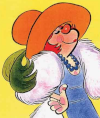
\includegraphics{foto_autor/borola-burron2.png} & \textbf{Ignacio Gran} Nació en el seno de una muy rica y reconocida familia de la Ciudad de México. Alega haber sido una gran vedette de los teatros, razonamiento que le permite no limitarse y explorar oficios tan diversos como piloto de carreras, luchadora enmascarada, médico cirujano o ingeniera empírica.
\end{tabular}
\end{center}
%----------------------------------------------------------------------------------------

\end{document}
